% Options for packages loaded elsewhere
\PassOptionsToPackage{unicode}{hyperref}
\PassOptionsToPackage{hyphens}{url}
\PassOptionsToPackage{dvipsnames,svgnames,x11names}{xcolor}
%
\documentclass[
  12pt,
  letterpaper,
  DIV=11,
  numbers=noendperiod]{scrartcl}

\usepackage{amsmath,amssymb}
\usepackage{lmodern}
\usepackage{iftex}
\ifPDFTeX
  \usepackage[T1]{fontenc}
  \usepackage[utf8]{inputenc}
  \usepackage{textcomp} % provide euro and other symbols
\else % if luatex or xetex
  \usepackage{unicode-math}
  \defaultfontfeatures{Scale=MatchLowercase}
  \defaultfontfeatures[\rmfamily]{Ligatures=TeX,Scale=1}
\fi
% Use upquote if available, for straight quotes in verbatim environments
\IfFileExists{upquote.sty}{\usepackage{upquote}}{}
\IfFileExists{microtype.sty}{% use microtype if available
  \usepackage[]{microtype}
  \UseMicrotypeSet[protrusion]{basicmath} % disable protrusion for tt fonts
}{}
\makeatletter
\@ifundefined{KOMAClassName}{% if non-KOMA class
  \IfFileExists{parskip.sty}{%
    \usepackage{parskip}
  }{% else
    \setlength{\parindent}{0pt}
    \setlength{\parskip}{6pt plus 2pt minus 1pt}}
}{% if KOMA class
  \KOMAoptions{parskip=half}}
\makeatother
\usepackage{xcolor}
\usepackage[margin=1in]{geometry}
\setlength{\emergencystretch}{3em} % prevent overfull lines
\setcounter{secnumdepth}{-\maxdimen} % remove section numbering
% Make \paragraph and \subparagraph free-standing
\ifx\paragraph\undefined\else
  \let\oldparagraph\paragraph
  \renewcommand{\paragraph}[1]{\oldparagraph{#1}\mbox{}}
\fi
\ifx\subparagraph\undefined\else
  \let\oldsubparagraph\subparagraph
  \renewcommand{\subparagraph}[1]{\oldsubparagraph{#1}\mbox{}}
\fi


\providecommand{\tightlist}{%
  \setlength{\itemsep}{0pt}\setlength{\parskip}{0pt}}\usepackage{longtable,booktabs,array}
\usepackage{calc} % for calculating minipage widths
% Correct order of tables after \paragraph or \subparagraph
\usepackage{etoolbox}
\makeatletter
\patchcmd\longtable{\par}{\if@noskipsec\mbox{}\fi\par}{}{}
\makeatother
% Allow footnotes in longtable head/foot
\IfFileExists{footnotehyper.sty}{\usepackage{footnotehyper}}{\usepackage{footnote}}
\makesavenoteenv{longtable}
\usepackage{graphicx}
\makeatletter
\def\maxwidth{\ifdim\Gin@nat@width>\linewidth\linewidth\else\Gin@nat@width\fi}
\def\maxheight{\ifdim\Gin@nat@height>\textheight\textheight\else\Gin@nat@height\fi}
\makeatother
% Scale images if necessary, so that they will not overflow the page
% margins by default, and it is still possible to overwrite the defaults
% using explicit options in \includegraphics[width, height, ...]{}
\setkeys{Gin}{width=\maxwidth,height=\maxheight,keepaspectratio}
% Set default figure placement to htbp
\makeatletter
\def\fps@figure{htbp}
\makeatother

% variáveis
\newcommand{\nome}{Alberson da Silva}
\newcommand{\sobrenome}{Miranda}
\newcommand{\titulo}{Relações Escolaridade-Renda no Espírito Santo}
\newcommand{\tituloingles}{Education-Income Relations in Espírito Santo}
\newcommand{\universidade}{Instituto Federal do Espírito Santo}
\newcommand{\campus}{Vitória}
\newcommand{\curso}{Licenciatura em Matemática}
\newcommand{\orientador}{Prof. Me. Diogo Oliveira}
\newcommand{\cidade}{Vitória}
\newcommand{\dia}{xx}
\newcommand{\mes}{dezembro}
\newcommand{\ano}{2022}
\newcommand{\grau}{Licenciado em Matemática}
\newcommand{\bancap}{Prof. Dr. Componente Banca}
\newcommand{\bancas}{Prof. Dr. Componente Banca}

% pacotes
\usepackage{bbm, times, quoting, setspace, lscape}
\usepackage{indentfirst, float, graphicx, psfrag, fancyhdr}
\usepackage{times, amsmath, amsfonts, amssymb, amsthm}
\usepackage{xcolor, url, placeins, sectsty, enumitem}
\usepackage{polyglossia, natbib, dcolumn}
\usepackage[T1]{fontenc}
\usepackage[skip = 2pt, size = normalsize]{caption}
\usepackage[labelfont = bf]{caption}

% fontes
\setmainfont{Times New Roman}
\setmonofont[Scale=0.9, Scale=MatchLowercase]{Consolas}
\sectionfont{\fontsize{12}{15}\selectfont}
\subsectionfont{\fontsize{12}{15}\selectfont}
%\renewenvironment{Shaded}
%    {\begin{snugshade}
%    \begin{singlespace}
%    \linespread{0.5}
%    }
%    {\end{singlespace}
%    \end{snugshade}
%}

% linguagem
\setdefaultlanguage{portuguese}
\deftocheading{toc}{}%
\deftocheading{lot}{}%
\deftocheading{lof}{}%

% cabeçalho e rodapé
\lhead{}
\chead{}
\rhead{\thepage}
\lfoot{}
\cfoot{}
\rfoot{}
\renewcommand{\headrulewidth}{0pt}

% espaçamento
\onehalfspacing
\linespread{1.5}

% ambiente citação
\newenvironment{citacao}
    {\begin{quoting}[rightmargin=0cm,leftmargin=4cm]
    \begin{singlespace}
    \footnotesize
    }
    {\end{singlespace}
    \end{quoting}
}

% legenda
\captionsetup[figure]{font=scriptsize}
\captionsetup{labelsep = endash, format = hang, width = \textwidth}

% posição das figuras
\floatplacement{figure}{H}
\floatplacement{table}{H}

% estilo
\pagestyle{fancy}

% bibliografia
\renewcommand{\bibsection}{}
\KOMAoption{captions}{tableheading}
\makeatletter
\makeatother
\makeatletter
\makeatother
\makeatletter
\@ifpackageloaded{caption}{}{\usepackage{caption}}
\AtBeginDocument{%
\ifdefined\contentsname
  \renewcommand*\contentsname{Table of contents}
\else
  \newcommand\contentsname{Table of contents}
\fi
\ifdefined\listfigurename
  \renewcommand*\listfigurename{List of Figures}
\else
  \newcommand\listfigurename{List of Figures}
\fi
\ifdefined\listtablename
  \renewcommand*\listtablename{List of Tables}
\else
  \newcommand\listtablename{List of Tables}
\fi
\ifdefined\figurename
  \renewcommand*\figurename{Figure}
\else
  \newcommand\figurename{Figure}
\fi
\ifdefined\tablename
  \renewcommand*\tablename{Table}
\else
  \newcommand\tablename{Table}
\fi
}
\@ifpackageloaded{float}{}{\usepackage{float}}
\floatstyle{ruled}
\@ifundefined{c@chapter}{\newfloat{codelisting}{h}{lop}}{\newfloat{codelisting}{h}{lop}[chapter]}
\floatname{codelisting}{Listing}
\newcommand*\listoflistings{\listof{codelisting}{List of Listings}}
\makeatother
\makeatletter
\@ifpackageloaded{caption}{}{\usepackage{caption}}
\@ifpackageloaded{subcaption}{}{\usepackage{subcaption}}
\makeatother
\makeatletter
\makeatother
\ifLuaTeX
  \usepackage{selnolig}  % disable illegal ligatures
\fi
\usepackage[]{natbib}
\bibliographystyle{apalike}
\IfFileExists{bookmark.sty}{\usepackage{bookmark}}{\usepackage{hyperref}}
\IfFileExists{xurl.sty}{\usepackage{xurl}}{} % add URL line breaks if available
\urlstyle{same} % disable monospaced font for URLs
\hypersetup{
  colorlinks=true,
  linkcolor={blue},
  filecolor={Maroon},
  citecolor={Blue},
  urlcolor={Blue},
  pdfcreator={LaTeX via pandoc}}

\author{}
\date{}

\begin{document}
\thispagestyle{empty}
\begin{center}
{\Large \MakeUppercase{\universidade\\ campus \campus\\ curso de \curso}}
\end{center}
\vspace{1cm}
\begin{center}
{\Large \MakeUppercase{\nome\>\sobrenome}}
\end{center}
\vspace{5cm}
\begin{center}
\Large \MakeUppercase{\textbf{\titulo}}
\end{center}
\vspace{5cm}

\begin{center}
\uppercase{\cidade}\\ \ano
\end{center}

\newpage
\thispagestyle{empty}
\setcounter{page}{1}

\begin{center}
{\Large \MakeUppercase{\nome\>\sobrenome}}

\vspace{6cm}

\Large \MakeUppercase{\textbf{\titulo}}

\normalsize

\vspace{3cm}
\end{center}

\hspace{7cm}{\begin{minipage}{8.5cm}{
Monografia apresentada à coordenadoria do curso de \curso\>do \universidade, Campus \campus, como requisito parcial para a obtenção do título de \grau.\\

Orientador: \parbox[t]{6.0cm}{\orientador}}
\end{minipage}}

\vspace{3cm}

\begin{center}
\cidade\\
\ano
\end{center}

\newpage
\thispagestyle{empty}

\begin{center}
{\large \MakeUppercase{\nome\>\sobrenome}}

\vspace{1cm}

\Large \MakeUppercase{\textbf{\titulo}}

\normalsize

\vspace{1cm}
\end{center}

\hspace{7.5cm}{\begin{minipage}{8.5cm}{
Monografia apresentada à coordenadoria do curso de \curso\>do \universidade, Campus \campus, como requisito parcial para a obtenção do título de \grau.\\}
\end{minipage}}

\vspace{1cm}

\hspace{9cm}

\uppercase{\textbf{Banca Examinadora}}

\vspace{1cm}
\begin{center}

\hspace{7cm}{\underline{\hspace{7cm}} \\}
\hspace{7cm}{\orientador \\}
\hspace{7cm}{\universidade}

\hspace{7cm}{\underline{\hspace{7cm}} \\}
\hspace{7cm}{\bancap \\}
\hspace{7cm}{\universidade}

\hspace{7cm}{\underline{\hspace{7cm}} \\}
\hspace{7cm}{\bancas \\}
\hspace{7cm}{\universidade}


\cidade, \dia\>de \mes\>de \ano.
\end{center}

\newpage
\thispagestyle{empty}
\begin{singlespace}
\noindent \MakeUppercase{\sobrenome}, \nome. \textbf{\titulo}. \ano. xx folhas. Monografia (\curso) -- \universidade, \cidade, \ano.

\vspace{1pc}
\begin{center}
\textbf{RESUMO}
\end{center}
\vspace{1pc}

\noindent
No máximo 500 palavras em espaço simples e sem parágrafos. Deve apresentar de forma concisa os objetivos, metodologia e os resultado alcançados, utilizar o verbo na voz ativa. Espaçamento simples, sem recuo de parágrafos.

\vspace{2pc}
\noindent
{\textbf{Palavras-chave}:}  Palavra 1. Palavra 2. Palavra 3. Palavra 4. Palavra 5.

\end{singlespace}

\newpage
\thispagestyle{empty}

\begin{singlespace}
\noindent \MakeUppercase{\sobrenome}, \nome. \textbf{\tituloingles}. \ano. xx folhas. Monografia (\curso) -- \universidade, \cidade, \ano.

\vspace{1pc}
\begin{center}
\textbf{ABSTRACT}
\end{center}
\vspace{1pc}

\noindent 
Tradução do resumo.

\vspace{2pc}
\noindent
{\textbf{Keywords}:}  Tradução das palavras chave.
\end{singlespace}

\newpage
\thispagestyle{empty}
\begin{flushleft}
\begingroup
\let\clearpage\relax

\newpage
\begin{center}
\MakeUppercase{\textbf{Sumário}}
\end{center}
\begin{center}
\tableofcontents
\end{center}
\end{flushleft}

\newpage
\thispagestyle{empty}
\begin{center}
\MakeUppercase{\textbf{LISTA DE FIGURAS}}
\end{center}
\begin{center}
\listoffigures
\end{center}

\newpage
\begin{center}
\MakeUppercase{\textbf{LISTA DE TABELAS}}
\end{center}
\begin{center}
\listoftables
\end{center}
\thispagestyle{empty}
\endgroup

\newpage

\hypertarget{introduuxe7uxe3o}{%
\section*{INTRODUÇÃO}\label{introduuxe7uxe3o}}
\addcontentsline{toc}{section}{INTRODUÇÃO}

\ldots{}

\hypertarget{resultados}{%
\section{RESULTADOS}\label{resultados}}

\begin{table}[!htbp] \centering 
  \caption{Estimação} 
  \label{} 
\footnotesize 
\begin{tabular}{@{\extracolsep{5pt}}lD{.}{.}{-3} D{.}{.}{-3} } 
\\[-1.8ex]\hline 
\hline \\[-1.8ex] 
 & \multicolumn{2}{c}{\textit{Dependent variable:}} \\ 
\cline{2-3} 
\\[-1.8ex] & \multicolumn{2}{c}{log(remuneração)} \\ 
 & \multicolumn{1}{c}{2019} & \multicolumn{1}{c}{2006} \\ 
\\[-1.8ex] & \multicolumn{1}{c}{(1)} & \multicolumn{1}{c}{(2)}\\ 
\hline \\[-1.8ex] 
 graudoutorado & 1.500^{***}$ $(0.026) & 1.700^{***}$ $(0.052) \\ 
  graufund\_I\_completo & 0.200^{***}$ $(0.017) & 0.290^{***}$ $(0.013) \\ 
  graufund\_I\_incompleto & 0.130^{***}$ $(0.017) & 0.210^{***}$ $(0.013) \\ 
  graufund\_II\_completo & 0.210^{***}$ $(0.017) & 0.300^{***}$ $(0.012) \\ 
  graufund\_II\_incompleto & 0.180^{***}$ $(0.017) & 0.250^{***}$ $(0.013) \\ 
  graumedio\_completo & 0.410^{***}$ $(0.016) & 0.550^{***}$ $(0.012) \\ 
  graumedio\_incompleto & 0.200^{***}$ $(0.017) & 0.360^{***}$ $(0.013) \\ 
  graumestrado & 1.400^{***}$ $(0.020) & 1.600^{***}$ $(0.025) \\ 
  grausuperior\_completo & 1.100^{***}$ $(0.017) & 1.400^{***}$ $(0.013) \\ 
  grausuperior\_incompleto & 0.630^{***}$ $(0.017) & 0.890^{***}$ $(0.013) \\ 
  sexofeminino & -0.300^{***}$ $(0.003) & -0.310^{***}$ $(0.003) \\ 
  raca\_coramarela & -0.088^{***}$ $(0.011) & -0.110^{***}$ $(0.012) \\ 
  raca\_corindigena & -0.048^{**}$ $(0.020) & -0.043^{***}$ $(0.016) \\ 
  raca\_corparda & -0.079^{***}$ $(0.002) & -0.035^{***}$ $(0.002) \\ 
  raca\_corpreta & -0.100^{***}$ $(0.003) & -0.056^{***}$ $(0.004) \\ 
  idade & 0.014^{***}$ $(0.0001) & 0.016^{***}$ $(0.0001) \\ 
  sexofeminino:raca\_coramarela & 0.083^{***}$ $(0.017) & 0.083^{***}$ $(0.020) \\ 
  sexofeminino:raca\_corindigena & -0.041$ $(0.029) & 0.029$ $(0.025) \\ 
  sexofeminino:raca\_corparda & 0.034^{***}$ $(0.003) & -0.025^{***}$ $(0.004) \\ 
  sexofeminino:raca\_corpreta & 0.041^{***}$ $(0.006) & -0.017^{**}$ $(0.007) \\ 
  Constant & 6.700^{***}$ $(0.017) & 5.600^{***}$ $(0.013) \\ 
 \hline \\[-1.8ex] 
Observations & \multicolumn{1}{c}{505,253} & \multicolumn{1}{c}{463,720} \\ 
R$^{2}$ & \multicolumn{1}{c}{0.320} & \multicolumn{1}{c}{0.310} \\ 
Adjusted R$^{2}$ & \multicolumn{1}{c}{0.320} & \multicolumn{1}{c}{0.310} \\ 
Residual Std. Error & \multicolumn{1}{c}{0.500 (df = 505232)} & \multicolumn{1}{c}{0.550 (df = 463699)} \\ 
F Statistic & \multicolumn{1}{c}{11,853.000$^{***}$ (df = 20; 505232)} & \multicolumn{1}{c}{10,456.000$^{***}$ (df = 20; 463699)} \\ 
\hline 
\hline \\[-1.8ex] 
\textit{Note:}  & \multicolumn{2}{r}{$^{*}$p$<$0.1; $^{**}$p$<$0.05; $^{***}$p$<$0.01} \\ 
\end{tabular} 
\end{table}

\hypertarget{referuxeancias}{%
\section{REFERÊNCIAS}\label{referuxeancias}}

\bibliography{config/bib.bib}

\newpage

\hypertarget{apuxeandice-a-a-escola-como-instituiuxe7uxe3o-panuxf3ptica}{%
\section*{APÊNDICE A: A ESCOLA COMO INSTITUIÇÃO
PANÓPTICA}\label{apuxeandice-a-a-escola-como-instituiuxe7uxe3o-panuxf3ptica}}
\addcontentsline{toc}{section}{APÊNDICE A: A ESCOLA COMO INSTITUIÇÃO
PANÓPTICA}

Em seu texto acerca dos Parâmetros Curriculares Nacionais --- PCN, o
professor Rômulo Lins abre da seguinte forma:

\begin{citacao}
Provavelmente o maior problema da educação matemática dos brasileiros não esteja nas atuais deficiências apontadas diversas vezes, tais como, por exemplo, formação inadequada de professores e abordagens inadequadas sendo levadas para as salas de aula. Parece-me que o maior
problema é a resistência do sistema em mudar. \citep{lins}
\end{citacao}

Para ele, a pesquisa relacionada às técnicas e abordagens em sala de
aula, o que ele chamou de \emph{micro}, não é suficiente para colocar o
sistema educacional em rota de mudança. Paralelamente, deve ser
realizado um trabalho estrutural na esfera \emph{macro} --- aqui,
principalmente, o MEC --- que possibilite uma mudança do educar
\emph{pela} matemática para o educar \emph{para} a matemática. Essa
diferença é ilustrada por Lins da seguinte forma:

\begin{citacao}
A diferença fica bastante mais clara se pensamos no caso da Educação Física. Será que alguém concebe que o papel das aulas de Educação Física é preparar todas as crianças (todas, eu disse) para o esporte competitivo? Claro que não. Se assim fosse as aulas de Educação Física não representariam, na formação das crianças, a educação para a saúde, para o desenvolvimento motor, para a socialização e o respeito a regras, para a colaboração. E os que quiserem ser atletas e jogadores vão buscar esta formação específica em outros espaços (possivelmente dentro dos times competitivos de suas escolas ou em clubes). Podemos dizer que a Educação Física escolar se concentra em modos de ser, promovendo aquela educação POR MEIO de esportes e exercícios físicos, enquanto o Treinamento Esportivo se concentra em potencializar habilidades, fazendo isso por meio da aquisição de técnicas específicas. \citep{lins}
\end{citacao}

A mudança, então, deixa de ter como meio apenas a sala de aula; o
problema norteador da educação matemática como disciplina deixa de ser
apenas, por exemplo, se o aluno deve ou não estudar geometrias não
euclidianas no ensino médio, ou seja, unicamente conteúdos, e se expande
para questionar o próprio objetivo do ensino da matemática, ou melhor,
\emph{através} da matemática.

Quando o autor propõe uma educação ``formativa e com o objetivo de
permitir que todos que passem por ela participem de forma plena em suas
sociedades'', podemos nos perguntar: o que é essa participação plena? Ou
ainda, por que é tão difícil realizar mudanças estruturais na educação
ou, como Lins diz, fazer com que o sistema se coloque em rota de
mudança? Podemos analisar essas perguntas sob a ótica da Sociologia da
Educação.

Em \emph{Sistemas de Ensino e Sistemas de Pensamento}, Pierre Bourdieu
coloca o sistema educacional como um dos instrumentos mais eficazes de
integração moral e lógica da sociedade, que tem como produto o indivíduo
``programado'' --- homogêneo em percepção, pensamento e ação:

\begin{citacao}
Caso se admita que a cultura e, neste caso particular, a cultura erudita em sua qualidade de código comum é o que permite a todos os detentores deste código associar o mesmo sentido às mesmas obras e, de maneira recíproca, de exprimir a mesma intenção significante por intermédio das mesmas palavras, dos mesmos comportamentos e das mesmas obras, pode-se compreender por que \textbf{a Escola, incumbida de transmitir esta cultura, constitui o fator fundamental do consenso cultural} nos termos de uma participação de um senso comum entendido como condição da comunicação. \citep{bourdieu}
\end{citacao}

Na conferência V de \emph{A Verdade e as Formas Jurídicas}, Foucault
coloca a escola como um exemplo de instituição panóptica (ou de
sequestro). Esse tipo de instituição exerce poder sobre os indivíduos em
uma sociedade de três formas características: \emph{vigilância}
individual e contínua; \emph{controle} através de punição e recompensa
e; formação e transformação dos indivíduos em função de certas normas, o
que Foucault chamou de \emph{correção}. Podemos associar esse consenso
cultural que Bourdieu trata ao tríplice aspecto das instituições
panópticas na definição de Foucault, especificamente a \emph{correção}.

\begin{citacao}
Na época atual, todas essas instituições --- fábrica, escola, hospital psiquiátrico, hospital, prisão --- têm por finalidade não excluir, mas, ao contrário, fixar os indivíduos. A fábrica não exclui os indivíduos; liga-os a um aparelho de produção. \textbf{A escola não exclui os indivíduos; mesmo fechando-os; ela os fixa a um aparelho de transmissão do saber}. O hospital psiquiátrico não exclui os indivíduos; liga-os a um aparelho de correção, a um aparelho de normalização dos indivíduos. O mesmo acontece com a casa de correção ou com a prisão. Mesmo se os efeitos dessas instituições são a exclusão
do indivíduo, elas têm como finalidade primeira fixar os indivíduos em um aparelho de normalização dos homens. A fábrica, \textbf{a escola}, a prisão ou os hospitais \textbf{têm por objetivo ligar o indivíduo a um processo de produção, de formação ou de correção dos produtores. Trata-se de garantir a produção ou os produtores em função de uma determinada norma}. \citep[p.~114]{foucault}
\end{citacao}

A primeira função da instituição panóptica é a extração da totalidade do
tempo do indivíduo. É preciso que todo o tempo da existência humana
esteja disponível ao trabalho, suas exigências ou sua preparação --- aí
incluindo a educação, que os economistas chamam frequentemente de
capital humano. Ao sequestrar o tempo do homem, ela transforma seu tempo
de vida em tempo de trabalho. A segunda função é controlar seus corpos,
fazendo com que o corpo do indivíduo se torne força de trabalho. Aqui o
corpo humano deve ser formado, reformado, corrigido. Deve ``adquirir
aptidões, receber um certo número de qualidades, qualificar-se como um
corpo capaz de trabalhar''.

A terceira função é a criação de um micro-poder político, econômico e
judiciário. A instituição panóptica se outorga o direito de decidir,
comandar, punir, recompensar e julgar. E a escola não passa
desapercebida:

\begin{citacao}
O sistema escolar também é inteiramente baseado em uma espécie de poder judiciário. A todo poder se pune e recompensa, se avalia, se classifica, se diz quem é o melhor, quem é o pior. [...] Por que, para ensinar alguma coisa a alguém, se deve punir e recompensar? Esse sistema parece evidente, mas, se refletirmos, vemos que a evidência se dissolve. \citep[p.~120]{foucault}
\end{citacao}

Por fim, a quarta função é a extração do saber, tanto a partir da
apropriação do conhecimento técnico e tecnológico produzido durante o
labor, quanto da observação do comportamento dos indivíduos vigiados e
controlados. Da mesma forma que as anteriores, essa função não é
restrita às relações sociais do capitalismo moderno:

\begin{citacao}
A pedagogia se formou a partir das próprias adaptações da criança às tarefas escolares, adaptações observadas e extraídas do seu comportamento para tornarem-se em seguida leis de funcionamento das instituições e forma de poder exercido sobre a criança. \citep[p.~122]{foucault}
\end{citacao}

Esse conjunto de características tem como objetivo principal a
\emph{transformação dos homens em força produtiva}. É através desse
micro-poder entranhado nas relações sociais de uma sociedade panóptica
que o indivíduo é fixado ao aparelho de produção, e a escola é um
instrumento essencial para a formação desse micro-poder.

Tendemos, por conta da brevidade de nossas vidas, a limitar nossa
ousadia em relação a essas estruturas. É fácil internalizar,
inconscientemente, que essas instituições sempre existiram e sempre
existirão da mesma forma que o são hoje. E talvez essa seja uma razão
que contribua para que, como aponta Lins, a produção na educação
matemática seja tão limitada à sala de aula --- aliás, essa visão é
incentivada aqui mesmo no IFES, onde somos direcionados a ``trazer para
a sala de aula'' nossa pesquisa do TCC.

Enquanto a educação exercer esse papel na sociedade, a sua estrutura é
inalterada na essência. Portanto, além de pensar no que Lins define como
micro e macro, devemos avançar acerca da própria posição da educação na
sociedade. Apenas no momento em que a escola não mais existir para
normalizar o indivíduo é que ela perderá sua razão de ser numa sociedade
panóptica capitalista e será livre para se tornar algo diferente --- e
de fato libertadora.

\newpage

\hypertarget{apuxeandice-b-derivauxe7uxe3o-dos-estimadores-de-mqo}{%
\section{APÊNDICE B: DERIVAÇÃO DOS ESTIMADORES DE
MQO}\label{apuxeandice-b-derivauxe7uxe3o-dos-estimadores-de-mqo}}

Partindo de um modelo de regressão linear simples,
\(Y_i = \beta_0 + \beta_1X_i + e_i\), em que \(e_i\) é o termo de erro
estocástico, em uma amostra, a relação \(Y\) e \(X\) é dada por:

\begin{enumerate}
\def\labelenumi{\arabic{enumi}.}
\item
  Função de regressão amostral \begin{equation}
  Y_i = \hat{\beta}_0 + \hat{\beta}_iX_i + \hat{e}_i
  \end{equation}
\item
  O valor \(Y_i\) previsto pelo ajuste \begin{equation}
  \hat{Y}_i = \hat{\beta}_0 + \hat{\beta}_iX_i
  \end{equation}
\item
  O resíduo \(\hat{e}_i\) não previsto pelo ajuste \begin{equation}
  \hat{e}_i = Y_i - \hat{Y}_i
  \end{equation}
\end{enumerate}

\begin{figure}

{\centering 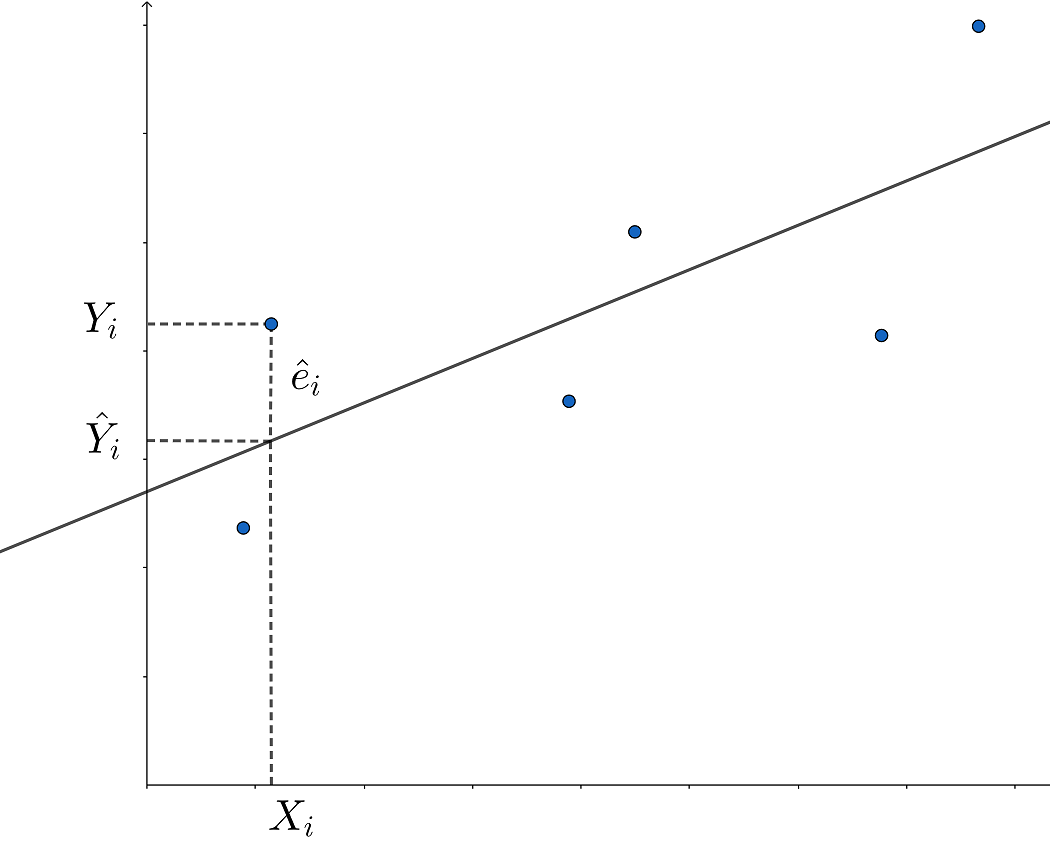
\includegraphics[width=0.7\textwidth,height=\textheight]{img/appendix_b_1.png}

}

\caption{Resíduo de ajuste}

\end{figure}

O objetivo é, portanto, estimar os coeficientes linear e angular que
representam a reta que minimiza os resíduos. Para essa função a ser
minimizada, posso utilizar tanto o erro absoluto \(\mid \hat{e}_i \mid\)
quanto o erro quadrático \(\hat{e}_i^2\). Por simplicidade, opto pelo
erro quadrático total.

\begin{equation}
\begin{aligned}
\text{EQT} & = \hat{e}^2_1 + \hat{e}^2_2 + ... + \hat{e}^2_n \\
& = (Y_1 - \hat{Y}_1)^2 + (Y_2 - \hat{Y}_2)^2 + ... + (Y_n - \hat{Y}_1)^2 \\
& = \sum_{i=1}^{n}(Y_i - \hat{Y}_i)^2 \\
& = \sum_{i=1}^{n}[Y_i - (\hat{\beta}_0 + \hat{\beta}_iX_i)]^2
\end{aligned}
\end{equation}

De posse da função, posso minimizar os coeficientes \(\beta_i\).
Considerando um modelo de regressão simples, posso estimar \(\beta_0\) e
\(\beta_1\) igualando as derivadas parciais à zero.

\begin{equation}
\begin{aligned}
\frac{\partial \text{EQT}}{\partial \beta_0} & = 2\sum_{i=1}^{n}[Y_i - (\hat{\beta}_0 + \hat{\beta}_1X_i)] (-1) & = 0 \\
& = -2 (\sum_{i=1}^{n} Y_i - \sum_{i=1}^{n} \hat{\beta}_0 - \sum_{i=1}^{n} \hat{\beta}_1X_i) & = 0 \\
& = \sum_{i=1}^{n} Y_i - n\hat{\beta}_0 - \hat{\beta}_1 \sum_{i=1}^{n} X_i & = 0 \\
& n\hat{\beta}_0 = \sum_{i=1}^{n} Y_i - \hat{\beta}_1 \sum_{i=1}^{n} X_i \\
& \hat{\beta}_0 = \frac{\sum_{i=1}^{n} Y_i - \hat{\beta}_1 \sum_{i=1}^{n} X_i}{n}
\end{aligned}
\end{equation}

\begin{equation}
\begin{aligned}
\frac{\partial \text{EQT}}{\partial \beta_1} & = 2\sum_{i=1}^{n}[Y_i - (\hat{\beta}_0 + \hat{\beta}_1X_i)] (-X_i) & = 0 \\
& = -2X_i (\sum_{i=1}^{n} Y_i - \hat{\beta}_0\sum_{i=1}^{n} - \hat{\beta}_1\sum_{i=1}^{n} X_i^2) & = 0 \\
\end{aligned}
\end{equation}



\end{document}
